\documentclass[12pt,a4paper]{article}
\usepackage[utf8]{inputenc}
\usepackage{amsmath}
\usepackage{listings}
\usepackage{verbatim}
\usepackage{graphicx} 
\oddsidemargin 0cm
\marginparwidth 0cm
\hoffset 0cm
\usepackage{polski}
\begin{document} 
\large
\begin{tabular}{|c|c|c|c|}
\hline
\multicolumn{4}{|l|}{Temat:}\\
\multicolumn{4}{|c|}{Wyznaczanie pierwiastków równania nieliniowego metodą Newtona}\\
\hline
\multicolumn{1}{|l}{Wykonał:}&\multicolumn{1}{|l}{Wydział:}&\multicolumn{1}{|c}{Kierunek}&\multicolumn{1}{|l|}{Grupa:}\\
Marcin Fabrykowski&FiIS&Inf. Stos.&grupa 3\\
\hline
\end{tabular}
\normalsize
\vspace{2cm}
\begin{enumerate}
\item Wstęp
Wyznaczanie pierwiastków równania nieliniowego metodą Newtona na wyznaczeniu przedziału izolacji danego pierwiastka. W~naszym przypadku wykonujemy to poprzez odczytanie przedziałów z~wykresu. Taki przedział oznaczamy poprzez $<a,b>$. Następnie wyznaczamy styczną do wykresu w~punkcie $b$. Równanie opisujące tą styczną: $$y-f(b)=f'(b)(x-b)$$
Przyjmujemy $y=0$ z~racji tego, że szukamy $x$ w~którym styczna przecina oś OX.$$x_1=b-\dfrac{f(b)}{f'(b)}$$
Następnie sprawdzamy czy $b-x_1<\varepsilon$. Jeśli powyższy warunek jest spełniony, wtedy przyjmujemy $x_1$ jako pierwiastek równania. W~przeciwnym wypadku przyjmujemy nowe $b=x_1$ i~powtarzamy procedurę.\\
Powyższy schemat powtarzamy dla wszystkich pierwiastków.
\item Wykonanie ćwiczenia.
Badamy funkcję:
$$f(x)=x^4-9x^3+29x^2-39x+18$$
Jej wykres przedstawia rys.~\ref{fig:wykres}\\
\begin{figure}
\caption{Wykres f(x)}
\label{fig:wykres}
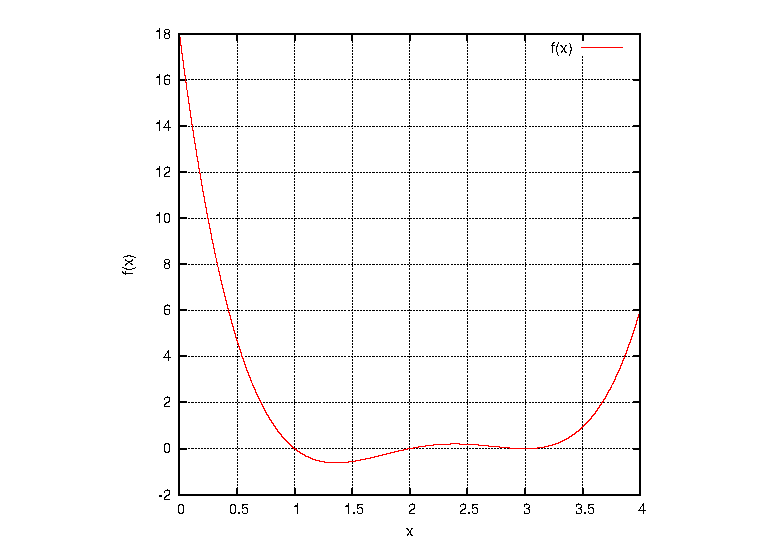
\includegraphics{f.eps}
\end{figure}
Zauważamy że przybliżone pierwiastki równania wynoszą: $1$,$2$ oraz $3$ dlatego przedziały izolacji wybieramy $\pm0.2$\\
Do wyliczenia pierwiastków wykorzystujemy własnoręcznie napisany program bazujący na algorytmie podanym we wstępie:
\lstinputlisting[language=C++,caption=main.cpp,breakatwhitespace=true,basicstyle=\footnotesize,breaklines=true]{main.cpp}
\item Wnioski
Dużą zaletą tej metody jest jest szybkość. Mianowicie liczba kroków potrzebnych do znalezienia pierwiastków jest niewielka, co pokazują dane wyjściowe:
\begin{enumerate}
\item dla pierwiastka pierwszego:
\verbatiminput{1.dat}
\item dla pierwiastka drugiego:
\verbatiminput{2.dat}
\item dla pierwiastka trzeciego
\verbatiminput{3.dat}
\end{enumerate}
Jednakże, wymagane jest podanie przedziałów izolacji pierwiastków, co nie jest ani wygodne, ani łatwe do wyznaczenia w~sposób automatyczny
\end{enumerate}
\end{document}
